\section{Game Combat Model}

\subsection{Modeling}

In order to search for a solution, we created the following components:

\begin{descri}
%STATE
\item[State] $s=<t,U,S_A,E>$:
\begin{shortitem}
\item Current game time $t$
\item Set $U$ of units  
\item Set $S_A$ of set of action that can be performed from $s$ ($S_A$ is a set of set of action)
\item Set of pending effect $E$ 
\end{shortitem}

%UNIT
\item[Unit] $u = <p,hp,b_a,b_m,b_c>$
\begin{shortitem}
\item Position $p = (x,y) \in \mathbb{R}^2$
\item Current hit point $hp$ ($\Leftrightarrow$ Health point)
\item Boolean indicating if unit can attack $b_a$, move $b_m$ or if its weapon is in cooldown $b_c$
\end{shortitem}

%ACTION
\item[Action] $a=<u,target,t_s,type>$
\begin{shortitem}
\item Unit $u$ to perform this action
\item Type $type$ of action:
    \begin{shortitem}
    \item Move to $target$
    \item Attack unit $target$
    \item \dots
    \end{shortitem}
    \item Time step $t_s$ when the action started
\end{shortitem}

%EFFECT
\item[Effect] $e=<u,target,t_e,type>$
\begin{shortitem}
\item Units $u$ and $target$ on which the effect applies 
\item Time step $t_e$ when the effect applies
\item Type $type$ of effect
    \begin{shortitem}
    \item Decrease $target.hp$
    \item Reset cooldown
    \item $u$ attacking (unable to move)
    \item \dots
    \end{shortitem}
\end{shortitem}
\end{descri}

Table \ref{effectUnits} presents the effect corresponding to an attack for two kind of units (a \texttt{Marine} and a \texttt{Firebat}).
As we can see deciding an action for a units has an impact in the \emph{future} frames.

\begin{table}[h!t]
\subfloat[$u$ being a \texttt{Marine} and $t_e = 0$]{
\centering
\begin{tabular}{cc|ccc}
&& $u$ can & Decrease & Weapon in \\
&& not move & $target.hp$ & cooldown \\
\hline
\multirow{4}{*}{\rot{Frame}} 
& 0    & \OK &     & \OK  \\
& 1    & \OK &     & \OK  \\
& 2-5  & \OK & \OK & \OK  \\
& 6-17 &     &     & \OK  \\
\end{tabular}
}
\\
\subfloat[$u$ being a \texttt{Firebat} and $t_e = 0$]{
\centering
\begin{tabular}{cc|ccc}
&& $u$ can & Decrease & Weapon in \\
&& not move & $target.hp$ & cooldown \\
\hline
\multirow{4}{*}{\rot{Frame}} 
& 0-4   & \OK &     & \OK  \\
& 5-6   & \OK & \OK & \OK  \\
& 7-10  & \OK &     & \OK  \\
& 11-24 &     &     & \OK  \\
\end{tabular}
}
\caption{Exemple of effects $e=<u,target,t_e,type>$}
\label{effectUnits}
\end{table}

\subsection{State generation}

Algorithm \ref{algGeneration} explains how a new state is constructed, taking in account the actions performed to go from the father to the new child and the pending effect.

\begin{figure}[h!t]
\begin{algorithm}[State generation]
The following algorithm describe how a state is constructed from its father.
In the following, $s_0$ denotates the father and $s_1$ the newly constructed state.

\begin{descri} 

% CASE ACTION AVAILABLE
\item[Case 1: A set $A_0$  of action can be performed from $s_0$]
\ \\
The new state $s_1=<t,U,S_A,E>$ is constructed as the following:
\begin{shortitem}
\item $s_1.t = s_0.t$ 
\item Apply the set of action $A_0$ to $s_0$ and create $s_1.E$:
\begin{align*}
s_1.E &= s_0.E \cup E_{A_0} \\
E_{A_0} &= \{\text{effect e | e was created by an action of } A_0\}  
\end{align*}
\item Create the set $S_{A}$ of set of actions avaible from $s_1$
\end{shortitem}
% CASE NO ACTION AVAILABLE
\item[Case 2: No actions can be performed from $s_0$]
\ \\
The new state $s_1 = <t,U,S_A,E>$ is constructed as the following:
\begin{shortitem}
\item $s_1.t = s_0.t + 1$
\item The new set of effect $s_1.E$ is:
\begin{align*}
s_1.E &= \{e \in s_0.E | e.t_e \geq s_1.t\}
\end{align*}
\item Create the set $S_{A}$ of set of actions avaible from $s_1$
\end{shortitem}
\end{descri}
\label{algGeneration}
\end{algorithm}
\end{figure}
When constructing the graph, all of the children can not be analysed. 
As an example, 8 units\footnote{Representing 4 vs 4 battle} with 6 possible actions (move \texttt{North}, move \texttt{South}, move \texttt{East}, move \texttt{West}, attack, hold) leads to $6^8 = 1679616$ possible combination for only the first frame. 
Therefore, only some path in the graph can be explored.
It is necessary to decide whether or not a state should be expanded.

Figure \ref{graph} display an example of a graph used by the algorithm. Only some nodes of the graph are contructed. Knowing \emph{where to go} in the graph depends of the algorithm used and is detailed in the following sections.
As shown in Algorithm \ref{algGeneration}, a child is generated either if there is actions available from the current state or by increasing the frame number.
As an example, assuming that our set of actions attributes an attack sequence to each of the \texttt{Marine} in the battleground and according to Table \ref{effectUnits}, there will not be any actions available until the next sixth frame.

\begin{figure}[h!t]
\centering
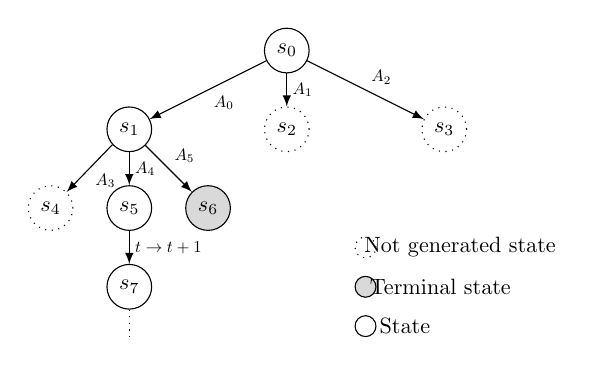
\begin{tikzpicture}[node distance = 1cm]
    \tikzstyle{node}=[circle,align=center,scale=0.8,draw]
    \tikzstyle{nodenotgen}=[circle,dotted,align=center,scale=0.8,draw]
    \tikzstyle{nodeterm}=[circle,fill=gray!30,align=center,scale=0.8,draw]
    \tikzstyle{link}=[->,thin,>=latex]
    
    \node[node] (s0) at (4,4) {$s_0$};

    \node[node] (s1) at (2,3) {$s_1$};
    \node[nodenotgen] (s2) at (4,3) {$s_2$};
    \node[nodenotgen] (s3) at (6,3) {$s_3$};

    \node[nodenotgen] (s4) at (1,2) {$s_4$};
    \node[node] (s5) at (2,2) {$s_5$};
    \node[nodeterm] (s6) at (3,2) {$s_6$};

    \node[node] (s7) at (2,1) {$s_7$};

    \node[auto,scale=0.8] (s8) at (2,0.2) {};
    
    \draw[link] (s0) to node [auto,scale=0.6] {$A_0$} (s1); 
    \draw[link] (s0) to node [auto,scale=0.6] {$A_1$} (s2);
    \draw[link] (s0) to node [auto,scale=0.6] {$A_2$} (s3);
    \draw[link] (s1) to node [auto,scale=0.6] {$A_3$} (s4);
    \draw[link] (s1) to node [auto,scale=0.6] {$A_4$} (s5);
    \draw[link] (s1) to node [auto,scale=0.6] {$A_5$} (s6);
    \draw[link] (s5) to node [auto,scale=0.6] {$t \rightarrow t+1$} (s7);
    \draw[-,>=latex,dotted] (s7) to (s8);
    

    %LEGEND

    \node[node] (l1) at (5,0.5) {}; % {$\phantom{s_1}$};
    \node[nodeterm] (l2) at (5,1)  {}; %{$\phantom{s_1}$};
    \node[nodenotgen] (l3) at (5,1.5) {}; %{$\phantom{s_1}$};
    \node[align=left,rectangle,scale=0.8] (l1t) at (5.5,0.5) {State};
    \node[align=left,rectangle,scale=0.8] (l2t) at (5.95,1.0) {Terminal state};
    \node[align=left,rectangle,scale=0.8] (l3t) at (6.2,1.5) {Not generated state};

\end{tikzpicture}
\caption{Exemple of a graph}
\label{graph}
\end{figure}


